\section{Conception\label{sec:conception}}

This chapter describes the solution concept and all aspects that were investigated to derive it.
The investigation includes the following activities:

First, the problem statement from Chapter \ref{sec:introduction} is revisited and further refined using information derived from concrete use cases, internal documents and from relevant literature.
Then, the elicited information is analyzed in detail to derive customization operations and criteria for the evaluation and selection of appropriate customization mechanisms that have been introduced in Chapter \ref{sec:foundation}. Finally, the solution concept is formalized.


\subsection{Refined problem statement}
The master's thesis aims to address the challenges of configuring simulations in the automotive industry through the use of semantic technology. The focus is on the development of an expert system that utilizes the metadata of existing simulations to facilitate the creation of new simulations. This solution aims to streamline the configuration process and make it more efficient and accessible, especially for inexperienced simulation engineers.

Here are a few use cases that can be derived from the problem raised by this thesis.

\begin{itemize}
    \item \textbf{New simulation configuration}: When a new simulation needs to be created, the system suggests relevant configurations based on previous simulations with similar goals or constraints, leveraging the semantic relationships embedded in the metadata. This can significantly reduce configuration time and ensure consistency with best practice.
    \item \textbf{Knowledge transfer}: The system serves as a knowledge repository that captures and stores information about previous simulations and their configurations. This allows new engineers to access valuable insights and learn from previous projects, shortening the learning curve and promoting knowledge sharing within the team.
    \item \textbf{Error prevention}: Semantic validation rules ensure that new configurations adhere to the defined guidelines and restrictions. This avoids errors and inconsistencies that could lead to inaccurate simulation results.
    \item \textbf{Configuration optimization}: The system can analyze previous simulation data and suggest optimized configurations based on performance metrics, allowing engineers to achieve better results with less effort.
\end{itemize}


\subsection{Simulation's Architecture}
Figure[] shows a general problem-solving diagram, illustrating how a problem might be handled using CAE methods. Above each phase is the sequence of different steps.\\

\begin{figure}[h]
    \centering
    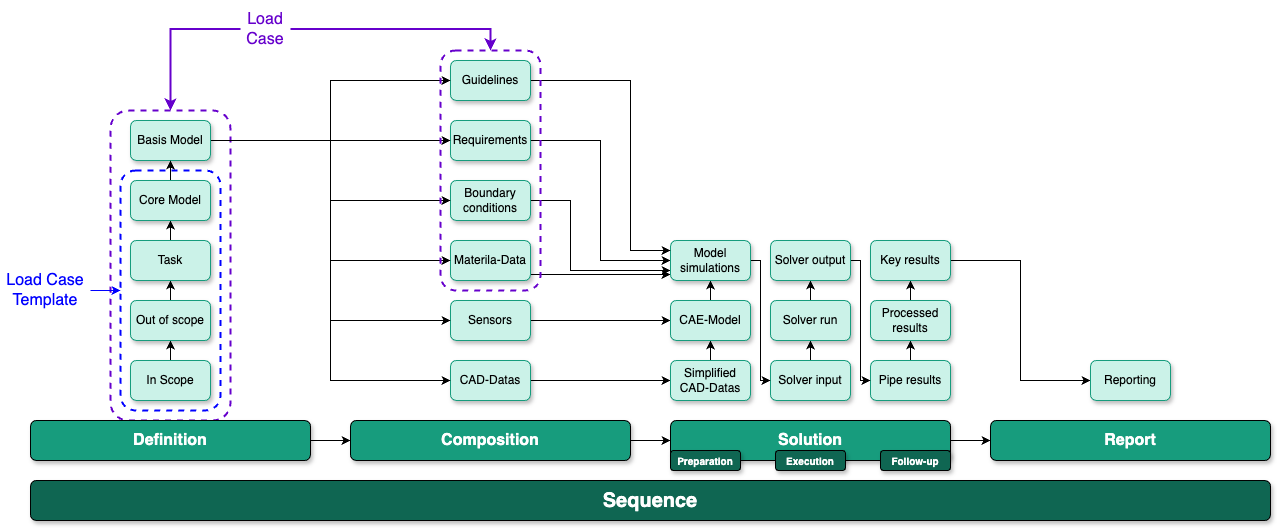
\includegraphics[width=\textwidth]{images/Concept-cae-process.drawio.png}
    \caption{\label{fig:cea-proc}  The CAE core process, illustrated with the stages of a general problem-solving scheme. [ ]}
\end{figure}

Based on the elements and steps involved in this process, a simulation ontology will be created. This will enable us to capture and formalize the elements involved in the configuration process, as well as the interdependencies between them. Particularly important in the context of this thesis are the elements involved in the “Definition” and “Composition” stages, as these lead to a "CAE-Model". Figure[] shows a UML diagram representing the information extracted from Figure[] and the relationships between them.\\

\begin{figure}[h]
    \centering
    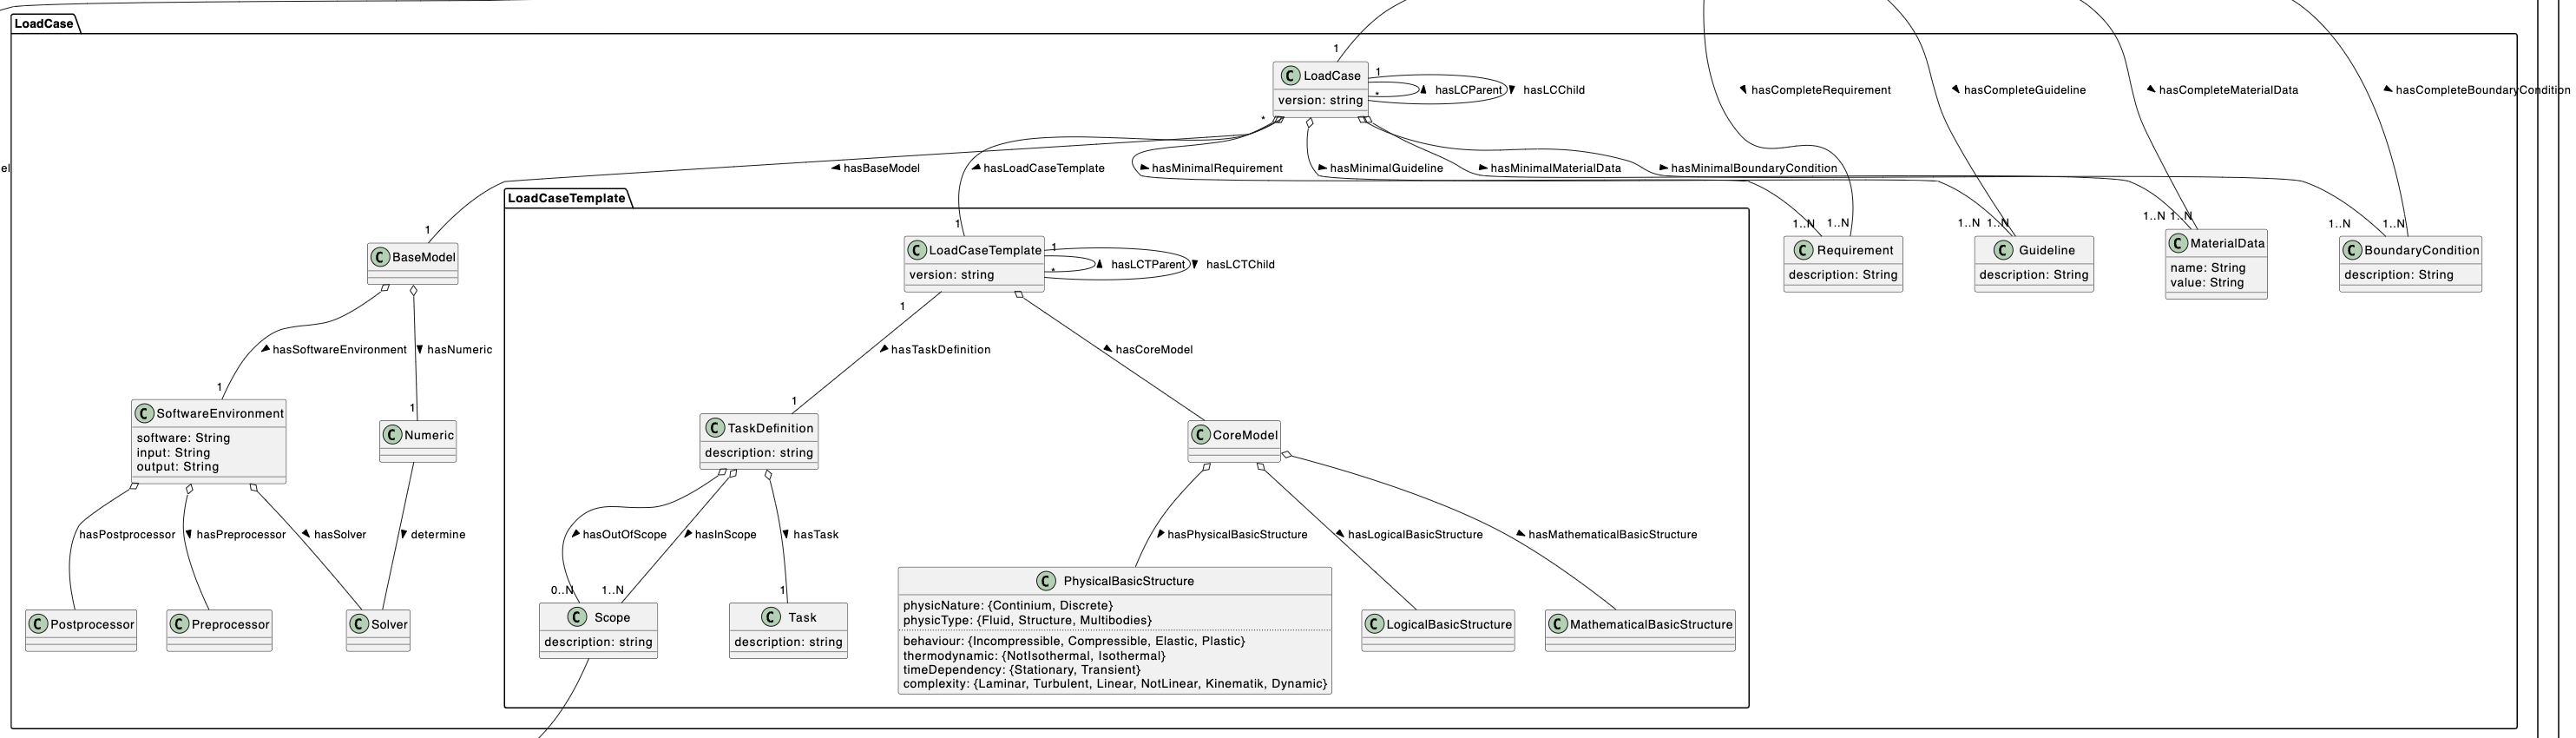
\includegraphics[width=\textwidth]{images/UML-Sim.png}
    \caption{\label{fig:uml-sim}  UML representation of the simulation’s metadata}
\end{figure}


\subsection{Simulation Modeling using Ontology}
There is no single technique for modeling a domain; there are always valid options. The ideal method is almost always determined by the application and extensions you intend to implement. Ontology development is an iterative process. Ontology concepts need to be linked to object (physical or logical) and relationships in your field of interest. These objects are most likely to be nouns (things) or verbs (relations) in the sentences describing your domain. As presented in Section\ref{subsec:sms_analysis}, the researchers behind the “Protégé” software have put together a set of best practices, which will be followed in this work []. The steps to follow are:

\begin{itemize}
    \item Step1: Scope Definition
    \item Step2: Reuse Existing Vocabulary
    \item Step3: Identification of Important Terms
    \item Step4: Class Hierarchy and Taxonomy
    \item Step5: Define Attributes and Properties of Classes — Slots
    \item Step6: Define the Facets of the Slots
    \item Step7: Creation of Instances
\end{itemize}

    \subsubsection{Step1: Scope Definition}
    The development of an ontology begins with the definition of its domain and field of application. To do this, few questions need to be answered []:
    
    \begin{itemize}
        \item What domain will the ontology cover? 
        \item For what purpose will we utilize the ontology? 
        \item To what kinds of queries should the knowledge in the ontology offer answers? 
        \item Who will utilize and maintain the ontology?
    \end{itemize}
    
    The answers to these questions have already been partially addressed in our previous analysis. In this thesis, an ontology will be created to model simulations and their metadata used during configuration. The aim of the ontology is to provide a formalism for the elements involved in the configuration process, and to model the relationships and interdependencies between these elements. Different simulation templates will be stored in the ontology, and information about them can be accessed using SPARQL queries (explained in Section\ref{para:sparql}). This will enable a suitable algorithm to provide assistance to future users. The ontology will be used primarily by simulation engineers. It will be maintained by an expert in semantic technology and expert simulation engineers, who will enrich it with their knowledge.

    
    \subsubsection{Step2: Reuse Existing Vocabulary}
    Setting up an ontology from scratch can be a rather tedious and complex process, requiring a certain level of knowledge in the target domain. That's why it's worth investigating whether there's a similar ontology to the one you want to build, which can be extended and refined to meet your requirements 100\%. Numerous ontologies are available in electronic form on the Internet. Platforms such as \textbf{DBPedia}, \textbf{WikiData} or \textbf{Linked Open Vocabularies (LOV)} allow you to access free ontologies, download them and integrate them into other ontologies.\\
    
    During the study in Chapter\ref{sec:relwork}, a number of simulation ontologies were identified. These include: OSMO [], I2Sim [], OntologySim[] and VIO[]. Unfortunately, given that the elements we want to model (see Figure\ref{fig:cea-proc}) come from conventions defined as part of the EP4.0 project [], it was impossible to find a free ontology that could cover our needs. The ontology will therefore have to be built from scratch, using the structure described in Figure\ref{fig:uml-sim}.


    \subsubsection{Step3: Identification of Important Terms}
    All the important terms can be extracted from the diagram in Figure[]. The most important are:
    \begin{itemize}
        \item LoadCase Template
        \item LoadCase
        \item Basic Model
        \item Core Model
        \item Numeric 
        \item Solver
        \item Physical Basic Structure
        \item Mathematical Basic Structure
        \item Logical Basic Structure
        \item Task
    \end{itemize}

    
    \subsubsection{Step4: Class Hierarchy and Taxonomy}
    There are three main techniques for building a class hierarchy.
    \begin{itemize}
        \item \textbf{A top-down development}: this method begins with the formulation of the most general notions of the domain, followed by the specialization of these concepts.
        \item \textbf{A bottom-up development}: this begins with the definition of the most detailed classes in the hierarchy, then groups these classes into more generic notions.
        \item \textbf{A combination development}: this method combines the two previous approaches. The most important ideas are first identified. They are then generalized and specified as appropriate.
    \end{itemize}
    
    For the purposes of this thesis, the third (hybrid) approach is the most appropriate. Since the majority of key elements have already been defined (top-down), it remains to group those of the same type into more generic notions (bottom-up). The various intermediates elements / classes are presented in the following diagrams:
    
    \begin{figure}
        \centering
            \begin{tikzpicture} 
            \centering
            \umlsimpleclass{Package} 
            \umlsimpleclass[x=-2, y=-2, anchor=north]{LoadCaseTemplate} 
            \umlsimpleclass[x=2, y=-2, anchor=north]{LoadCase} 
            \umlVHVinherit[arm2=-1.2cm]{LoadCaseTemplate}{Package} 
            \umlVHVinherit[arm2=-1.2cm]{LoadCase}{Package} 
            \end{tikzpicture} 
        \caption{\label{fig:distro-art} Classification of “Package”}
    \end{figure}
    
    \begin{figure}
        \centering
            \begin{tikzpicture} 
            \centering
            \umlsimpleclass{Model} 
            \umlsimpleclass[x=-2, y=-2, anchor=north]{BasicModel} 
            \umlsimpleclass[x=2, y=-2, anchor=north]{CoreModel} 
            \umlVHVinherit[arm2=-1.2cm]{BasicModel}{Model} 
            \umlVHVinherit[arm2=-1.2cm]{CoreModel}{Model} 
            \end{tikzpicture} 
        \caption{\label{fig:distro-art} Classification of “Model”}
    \end{figure}
    
    \begin{figure}
        \centering
            \begin{tikzpicture} 
            \centering
            \umlsimpleclass{BasicStructure} 
            \umlsimpleclass[x=-2, y=-2, anchor=north]{PhysicalBasicStructure} 
            \umlsimpleclass[x=4, y=-2, anchor=north]{MathematicalBasicStructure}  
            \umlsimpleclass[x=10, y=-2, anchor=north]{LogicalBasicStructure} 
            \umlVHVinherit[arm2=-1.2cm]{PhysicalBasicStructure}{BasicStructure} 
            \umlVHVinherit[arm2=-1.2cm]{MathematicalBasicStructure}{BasicStructure} 
            \umlVHVinherit[arm2=-1.2cm]{LogicalBasicStructure}{BasicStructure} 
            \end{tikzpicture} 
        \caption{\label{fig:distro-art} Classification of “BasicStructure”}
    \end{figure}
    

    
    \subsubsection{Step5: Define Attributes and Properties of Classes — Slots}
    In order to achieve a complete, connected knowledge model, the properties of the various classes and the relationships between these classes still need to be explicitly defined. Here again, our UML diagram in Figure\ref{fig:uml-sim} comes into play. It contains the definition of each class and their properties.
    
    
    \subsubsection{Step6: Define the Facets of the Slots}
    Slots can have many facets that describe the type of value, the permitted values, the number of values (cardinality) and other characteristics of the values the slot can accept. A facet can be a string, a number, a Boolean literal or an instance of a class. The “range” represents the classes authorized for the value of a property. And the “domain” represents the classes that a property can describe. The diagram in Figure\ref{fig:uml-sim} also shows the relationships between the various classes, as well as their cardinalities.
    
    
    \subsubsection{Step7: Creation of Instances}
    For our purposes, instances will be created using a migration system when our server is first launched (see Chapter\ref{sec:implementation}).
    

\subsection{Case-Based reasoning \label{subsec:cbr}}
Case-based reasoning (CBR) is an approach to building intelligent systems that models the way humans think. Figure\ref{fig:simple-cbr} shows a simplified model of CBR. This method involves recording past experiences in the form of cases. These cases are then retrieved and reused (partially, fully or modified) to solve new problems. The new experience acquired in this way will in turn be stored in the memory and will later help in the resolution of a new case. It's therefore a cycle following a number of stages. Figure\ref{fig:cbr-cycle} shows the CBR cycle. And the stages making up this cycle are as follows.
    
    \begin{enumerate}
        \item Retrieve
        \item Reuse
        \item Revise
        \item Retain
    \end{enumerate}
    
    \begin{figure}[h]
    \centering
    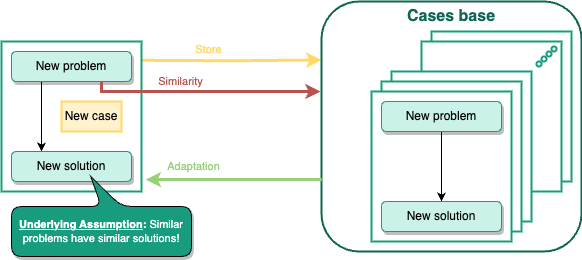
\includegraphics[width=\textwidth]{images/Concept-simplified-cbr-Simplified CBR princip.drawio.png}
    \caption{\label{fig:simple-cbr}  Simplified model of CBR []}
    \end{figure}
    
    \begin{figure}[h]
    \centering
    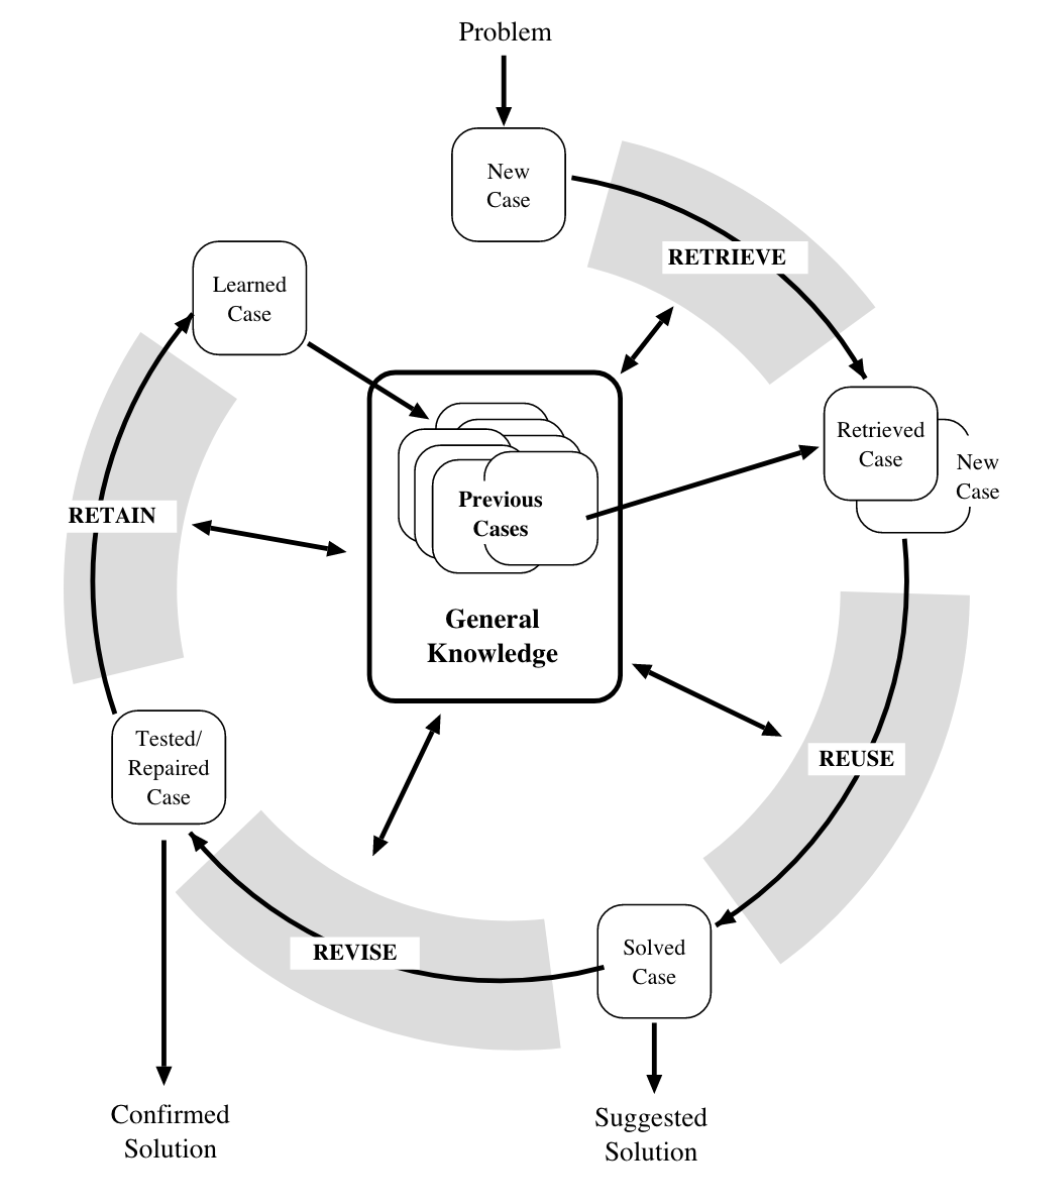
\includegraphics[scale=0.6]{images/Concept-cbr-cycle.png}
    \caption{\label{fig:cbr-cycle}  CBR cycle []}
    \end{figure}
    

    \subsection{Retrieve}
    The aim here is to find the case(s) in the database most similar to the query, taking into account certain similarity functions or criteria. The key question here is how to measure similarity between 2 entities. This will be studied in greater depth in Section\ref{parag:similarity}. The problem that can quickly arise here is that, over time, as the database of cases increases, the efficiency of the search decreases. This is because numerous cases have to be examined to find the most similar ones. There is therefore a sub-field of CBR research which focuses on methods to improve search efficiency. One example is the use of special index structures such as "kd-trees", case-finding networks or discrimination networks [ ].
    
    \subsection{Reuse}
    Once similar cases have been obtained, the answer (or any other information relating to the solution of the problem) from these cases is used to deal with the current problem. There are two types of reuse: simple reuse and reuse with adaptation. 
    
    \begin{itemize}
        \item \textbf{Simple reuse} involves using the recovered answer as a suggested solution for the new problem, without modification. This method is much better suited to classification work, which involves a few solutions but many cases.  For this scenario, all potential solutions are already present in the case base, so adaptation is generally not necessary. 
        
        \item \textbf{Reuse with adaptation} is necessary for synthetic tasks such as planning or configuration. For these tasks, the number of possible solutions far exceeds the number of available examples (or is even infinite).
    \end{itemize}

    Numerous adaptation proposals have been put forward within the CBR framework. The main difference between all these adaptation methods is whether they are transformational or generative.
    
    \begin{itemize}
        \item Transformational adaptation is based on a set of adaptation rules or operators, which specify how variations in the problem lead to the necessary changes in the solution.  
        
        \item Generative adaptation requires the use of a generative problem solver such as LLM. The latter must be able to solve problems based on general knowledge. Here, it's not the case solutions that are really used, but the path (reasoning) taken to obtain these solutions. 
    \end{itemize}

    Adaptation can be a tedious process. This is why the majority of work in the field of CBR seeks to avoid or reduce the modifications to be made once an interesting case has been obtained.


    \subsection{Revise}
    This stage provides feedback on the solution. The aim is to determine whether the solution works and is relevant, through verification in simulations or in the real world. This feedback can take the form of an accuracy score.
    
    
    \subsection{Retain}
    This phase represents the learning phase of the CBR system. In a CBR system, learning consists in adding a new case, generally by modifying a case already in the case base. This new case then becomes available for use in future problem-solving processes.\\
    However, as mentioned above, the constant expansion of the case base can at some point create a utility problem, as it reduces the efficiency of the search. Researchers have devised special algorithms for learning similarity measures. Early techniques focused on the use of feature weights [ ]. But more recent methods tackle the more difficult task of using local and global similarity functions [ ]. 

    
    
    \subsection{Similarity\label{subsec:similarity}}
    As presented in the retrieve step, the main concept of CBR is similarity. This is due to the fact that the cases chosen during the process are those most similar to the current situation (query). Similarity can be formalized by a function $sim: P \times P \rightarrow [0, 1]$, which compares two problem descriptions of type \textbf{P} and returns a score between 0 and 1. The higher this score, the more similar the two problems are considered to be [ ].\\
    For a new problem \textbf{p}, a case $c_1 = (p_1, s_1)$ is more appropriate than a case $c_2 = (p_2, s_2)$ (represented by $c_1 \succ_p c_2$) \textbf{iff} $sim(p, p_2) < sim(p, p_3)$. Here, the exact value of the similarities is not the most important factor, but the fact that these values allow us to give an order of relevance between the different cases considered. This order of preference corresponds to the evaluation of the usefulness of these cases for the treatment of problem \textbf{p} during the reuse phase.\\
    
    The local-global approach, first introduced by Richter [ , ], is the most widely implemented. Figure\ref{fig:cbr-exam} shows an example of similarity calculation using this principle. Here, cases are represented by graphs, in which each \textbf{Node} has attributes $A_i$ of different types $T_i$. For each Node, a local calculation is first performed at the level of these attributes, using a similarity function $_i = sim_{A_i} : T_i \times T_i$ according to the type of attribute. The local similarities are then combined to calculate the global similarity using an appropriate combination. The combination adopted is called the \textbf{amalgamation function: F}, and also takes into account the different weights of the attributes. There are a number of different amalgamation functions:
    \begin{itemize}
        \item \textbf{Weighted Average}: $F(s_1,...,s_n)= \sum_{1=1}^{n} w_i*s_i$
        \item \textbf{Maximum}: $F(s_1,...,s_n) = max\{s_1,...,s_n\}$
        \item \textbf{k-Minimum}: $F(s_1,...,s_n) = s_{ik} \quad with \quad s_{i1} \leq s_{i2} \leq ... \leq s_{in}$
    \end{itemize}
    
    The global similarity can therefore be described mathematically as follows:\\
    \[sim(x,y) = sim((x_1,...,x_n),(y_1,...,y_n)) = F(sim_{A_1}(x_1, y_1),..., sim_{A_n}(x_n, y_n) )\] where \[F: [0,1]_n \rightarrow [0,1]\].\\


    \begin{figure}[h]
    \centering
    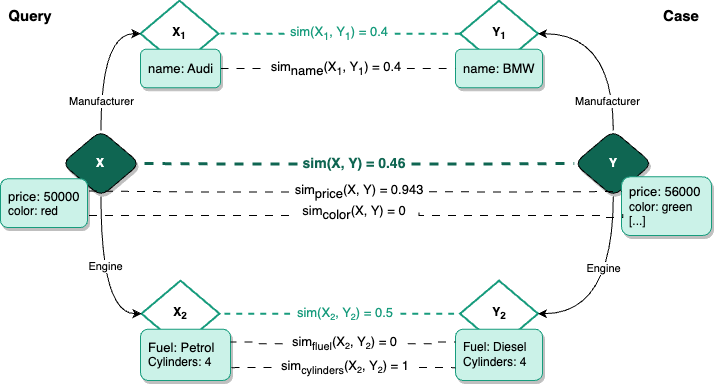
\includegraphics[scale=0.6]{images/Concept-CBR Exemple.drawio.png}
    \caption{\label{fig:cbr-exam}  Calculation of similarity using the local-global principle}
    \end{figure}
    
    \begin{itemize}
        \item $sim_{price}$ is calculated using a \textbf{linear numerical measurement}. The function used is $(n_1, n_2) \rightarrow 1 - abs(n_1 - n_2) / (n_1 + n_2)$. This gives a value of 0.943
        \item for $sim_{color}$ the \textbf{string equality measure} is used. Since \textbf{red != green} the obtained value is 0.
        \item $sim_{fuel}$ is calculated using a string equality measure. Since \textbf{Petrol != Diesel} we obtain a value of 0
        \item $sim_{cylinder}$ is calculated using linear numeric measure. Since they two values are equal, we have a similarity of 1.
        \item $sim(X_2, Y_2)$ is obtained by aggregating the similarities of the Fuel and Cylinders attributes with equal weighting. $sim(X_2, Y_2) = \frac{1}{2} * 0 + \frac{1}{2} * 1 = 0.5$
        \item $sim_{name}$ is calculated using a \textbf{taxonomic similarity measure} based on a semantic taxonomy (Bergmann 2002)[].
        \item $sim(X_1, Y_1) = 1 * 0.4 = 0.4$
        \item finally $sim(X, Y) = \frac{1}{4} sim_{price} + \frac{1}{4} sim_{color} + \frac{1}{4} sim(X_1, Y_1) + \frac{1}{4} sim(X_2, Y_2) = 0.46$

    \end{itemize}

